DaisyNFS is a verified, concurrent, and crash-safe file system, built on top of
GoTxn. This chapter describes its specification, implementation, and proof. A
key aspect of DaisyNFS is that the proofs of the file-system code use \emph{sequential
reasoning}, even though DaisyNFS is a concurrent file system --- this is possible
due to a \emph{simulation-transfer theorem}. The theorem uses the strong
guarantee of GoTxn to enable verifying a system written with transactions using
entirely different techniques, so that the file-system proofs are carried out in
Dafny, a sequential verification-oriented programming language.

\section{Introduction}

File systems are important to implement correctly because applications rely on
them to safely store user data. Formal verification offers a promise of showing
that an implementation always meets its specification, including a crash safety
property that says the file system recovers correctly from a sudden crash and
reboot. However, efficient implementations are internally complicated,
especially because they support concurrency and aim to minimize disk writes.
This poses a challenge for formal verification: how can a proof cover
concurrency, crash safety, and functional behavior while remaining tractable for
a program the size of a file system?

Crash safety poses a challenge even without verification, so many file systems
use a technique called \emph{journaling} (sometimes called write-ahead logging)
to atomically write multiple objects to disk. An efficient journaling system
goes a long way towards correctness, but it does not protect the programmer from
all concurrency and crash safety reasoning. For example, consider allocating a
block using a combination of an in-memory allocator an on-disk state (to recover
the allocator state on reboot). Suppose one operation is freeing a block from a
file while a concurrent operation is allocating and using it. If the system
crashes, it is possible that the allocation and its writes succeed but the
freeing is aborted, resulting in the same block being part of two files.

The main contribution of this paper is a file-system design that \emph{isolates
crash safety and concurrency reasoning} to a transaction-system
implementation. We take inspiration from databases, which provide SQL
transactions to applications to avoid such tricky concurrency and crash
reasoning when using the database, except in this case the transactions help the
file-system implementation safely access the disk. Unlike existing designs, we
wrap all the file-system data structures and logic inside a transaction. The
benefit of this design is that it is especially verification friendly since it
supports \emph{sequential proofs} for the body of each transaction. Sequential
proofs keep the proof burden manageable even with an efficient implementation
which supports many features, such as large files and in-place updates of
serialized metadata.

There are two challenges in realizing this design. First, how can the entire
file system be implemented using transactions? Ordinarily file systems have some
shared mutable state that is independent of the journal --- the allocator is one
such piece of state that gives rise to the running bug example. We address this
issue by not relying on atomicity of the allocator and instead validating its
results with the journal (experiments demonstrate this has only a small
performance impact). Some operations, like freeing, can require a large number
of disk writes that might not fit in a transaction. We implement freeing using
multiple transactions; a first transaction logically deletes a file, and then
asynchronously the implementation can run transactions that recover space from
the file but have no other visible effect.

The second challenge is how to implement and prove the transaction system
itself. The performance and concurrency of the overall system can only be as
good as the transaction system, so efficiency and fine-grained locking are
important. To that end we start with GoJournal~\cite{chajed:gojournal}, a
verified journaling system that gets good performance and supports concurrent
access to objects smaller than the disk's block size (assumed to be 4KB).
GoJournal leaves concurrency control to the caller, which our transaction system
implements using a standard two-phase locking implementation.

There are two difficulties in proving the transaction system correct using the
GoJournal specificationh. First, this implementation cannot make all
transactions appear sequential; consider a simple example of a transaction that
increments a global variable unknown to the two-phase locking code. Instead, we
formalize a contract specifying rules for which transactions are legal and
assume the caller issues legal transactions in the correctness proof. Second,
most textbook proofs of two-phase locking work by showing that a global conflict
graph between transactions is cycle-free, which implies that the transactions
are serializable. Our proof needs to be tied to the implementation and in
particular the GoJournal specification based on separation logic, so we give a
new proof of two-phase locking's correctness using lock invariants and local
rather than global reasoning.

The verified artifact from this work is \sys, which implements a Network File
System (NFS) server on top of a bare disk and comes with a proof that clients
observe that each operation follows the NFS specification as laid out in RFC
1813. Operations appear atomic despite concurrency and crashes. Clients can use
the Linux or macOS NFS client to mount \sys like any other file system and
interact with it using the usual POSIX API.
As an end-to-end check that our formalization of NFS is
accurate and the implementation is reasonably complete, we tested with both Linux
and macOS clients running a variety of programs and under interactive usage.

A significant benefit of this file-system design is that it permits using the
sharpest tool for each part of the proof: while we use
Perennial~\cite{chajed:gojournal}, a program logic for crash safety and concurrency, for the
transaction system's proof, we use Dafny~\cite{leino:dafny}, a verification-aware
programming language with powerful automation, for the file-system operations.
Dafny is a purely sequential language, but we are able to use it despite this
limitation since the transaction system's proof guarantees transactions behave
sequentially. The value of
sequential proofs can be seen in the proof-to-code ratio for the transaction
system, which is $18\times$, versus the Dafny proofs which required about
$2\times$ as many lines of proof as code. Further evidence can be seen in the
incremental development of DaisyNFS, which we elaborate on in
\autoref{sec:eval:incremental}.

% \joe{Should some of this paragraph's ideas move up to the part where we first argue for the split and describe Dafny as the best tool for the other side?}
% The verification approach we propose makes the proof much simpler. The
% productivity from doing the proofs in Dafny enabled us to rapidly prototype and
% add features incrementally, including triply-indirect blocks, directories, and
% efficient in-memory data structures. These features were important to get good
% performance and support a range of applications. As some quantitative evidence
% for simpler proofs, \sys's \sys's proof is about $2\times$ as many lines as its
% implementation, a rough measure of proof complexity. For comparison, this is
% significantly lower than the overhead in our transaction system (about
% $18\times$) and comparable to the proof:code ratio for the three prior systems
% verified in Dafny, IronClad~\cite{hawblitzel:ironclad} with $4.8\times$,
% IronFleet~\cite{hawblitzel:ironfleet} with $3.6\times$, and VeriBetrKV~\cite{hance:veribetrkv} with
% $4\times$.\footnote{These numbers exclude refinement proofs in these systems
% written on top of the implementation specs, since \sys does not have any
% comparable proofs.}

To evaluate DaisyNFS's performance, we compare it to that of the Linux NFS server
exporting an ext4 file system. \sys achieves almost the same performance as
Linux with the ext4 \cc{data=journal} option (which gives the same crash-safety
guarantees as \sys), across a variety of benchmarks run on top of a fast NVMe
drive. The comparable performance is due to the efficiency of GoJournal and
adding little overhead in the file-system code (e.g., updating data structures
in place to avoid copying). We do note that ext4's default \cc{data=ordered}
mode can get about $2\times$ better throughput for data-heavy workloads, at the
cost of relaxed guarantees on crash.

The contributions of this paper are:
\begin{itemize}
  \item A file-system design that uses transactions in a principled way to
  isolate crash safety and concurrency to the transaction system and use
  sequential proofs for file-system logic.
  \item A contract formalizing which transactions the transaction system can
  make atomic, and a proof of its correctness under this contract.
  \item DaisyNFS, a verified file system and transaction system that implement
  these ideas. A performance evaluation shows that DaisyNFS gets performance
  comparable to Linux ext4 exported over NFS.
\end{itemize}

Our approach and DaisyNFS have some limitations. We do not support NFS unstable
writes, which improve performance by not committing writes to stable storage
until explicitly requested. The proof approach relies on showing that
transactions appear to execute sequentially; this prevents us from modifying state
outside the transaction system (and reasoning about the interaction) where that
would get better performance. The transaction system does not have a proof of
liveness, and we do not prove that transactions avoid deadlock. Our NFS
implementation does not cover the entire API, such as symbolic and hard links,
the ``weak-cache consistency'' metadata to support client-side caching, or
paginated \cc{READDIR}; we believe all of these could be implemented and
specified with the same approach, but have not done so in our prototype.

\section{System design}%
\label{sec:system}

% \begin{figure}
%   \center
%   \includegraphics{drawn-diagrams/system-overview.png}
%   \caption{The structure of the code.}
%   \label{fig:system}
% \end{figure}

\begin{figure}
  \center
  \begin{tikzpicture}[>=latex, node distance=1.25cm]

 \tikzset{
    genericnode/.style={rectangle,draw,minimum width=2cm, minimum height=.85cm, align=center,},
    layer/.style={
      genericnode,
      alias=genericnode,% <- alias added
      label={[anchor=south west,shift={(genericnode.north west)},inner sep=2pt]{\tiny #1}}% position the label using the alias
    }}

%\tikzstyle{layer}=[rectangle, draw, minimum width=2cm, minimum height=.85cm, align=center];
\tikzstyle{genlayer}=[dashed, layer={}];
\tikzstyle{edge}=[->,thick];

\draw node (dispatch) [layer=Go] {Dispatch Loop};
\draw node (goout) [genlayer,below of=dispatch] {Go output};
\draw node (txn) [layer=Go,below of=goout] {GoTxn};

\draw node (coq) [left=1.5cm of txn, align=center] {Verification \\ in Perennial};
\draw node (dafny) [left=1.25cm of goout, layer=Dafny] {File-system \\ Operations};

\draw node (out) [below=1cm of txn] {\texttt{daisy-nfsd} binary};

\draw [thick] (dispatch.south) -- (goout.north);
\draw [thick] (goout.south) -- (txn.north);
\draw [edge] (txn.south) -- node[right] {\texttt{go build}} (out.north);
\draw [edge] (txn.west) -- (coq.east);

\draw [edge] (dafny.east) -- node[above] {\texttt{dafny}} (goout.west);


\end{tikzpicture}

  \caption{The structure of the code.}
  \label{fig:system}
\end{figure}

As shown in \autoref{fig:system}, \sys is implemented in three layers:
1) a dispatch loop that speaks the NFS wire protocol and calls the
appropriate method for each operation; 2) a Dafny class that
implements each method; and 3) a transaction system that applies the
updates of each method to the disk atomically.  The dispatch loop is
unverified; we assume that the server correctly decodes messages,
calls the right method for an operation, and encodes the response. The
middle layer implementing the file-system operations is implemented
and verified in Dafny, which has a backend for Go.  The
third layer is directly written in Go and verified using Coq and
Perennial.  By implementing the file system on top of the transaction
system, we can implement each NFS method in Dafny as sequential code
calling into a concurrent transaction system library. The NFS
operations supported by \sys are listed in \autoref{fig:nfs}.

\subsection{Dafny file system}

%% We focus on the
%% design of the transaction system here, but the file system also has several
%% internal abstractions. These abstractions are primarily interesting in a
%% verification context so we discuss them later in \autoref{sec:design}.

%% The file-system implementation calls the transaction system to store all
%% file-system data, ensuring that it is written atomically and durably.

% \begin{figure}
%   \begin{center}
%   \includegraphics[width=\columnwidth]{drawn-diagrams/disk-layout.png}
%   \end{center}
%   \caption{The layout of the file system on top of the transaction system's
%     disk. The number of inode blocks and data bitmap blocks is a compile-time
%     constant, but easy to change without affecting the proofs.}
%   \label{fig:layout}
% \end{figure}

\begin{figure}
  %\includegraphics[width=\columnwidth]{drawn-diagrams/disk-layout.png}
  \begin{tikzpicture}[>=latex]

  \tikzstyle{circlog}=[thick,rectangle, draw,minimum height=1cm, align=center];

  \node[circlog,minimum width=1cm,
       label={[label position=below, align=center]Super\\block}] (logger) {};
  \node[circlog,minimum width=1.7cm, right=0cm of logger,
    inner sep=0pt,
    rectangle split,
    rectangle split every empty part={},
    rectangle split parts=6,
    rectangle split empty part width={.2cm},
    rectangle split horizontal,
       label={[label position=below, align=center]20 inode\\ blocks}] (installer) {};

  \node[circlog, right=0cm of installer,
    inner sep=0pt,
    rectangle split,
    rectangle split every empty part={},
    rectangle split parts=20,
    rectangle split empty part width={.1cm},
    rectangle split horizontal,
       label={[label position=below, align=center]30 allocator\\ bitmap blocks}] (log) {};


  \node[circlog,minimum width=3.2cm, right=0cm of log,
    inner sep=0pt,
    rectangle split,
    rectangle split every empty part={},
    rectangle split parts=3,
    rectangle split empty part width={1.15cm},
    rectangle split horizontal,
       label={[label position=below, align=center]data blocks\\ (remainder of disk)}] (log2) {};

  \draw [line width=.05cm,black,transform canvas={yshift=.25cm}] (installer.south west)+(0,-.5cm) -- (installer.north west);
  \draw [line width=.05cm,black,transform canvas={yshift=.25cm}] (log.south west)+(0,-.5cm) -- (log.north west);
  \draw [line width=.05cm,black,transform canvas={yshift=.25cm}] (log2.south west)+(0,-.5cm) -- (log2.north west);

%  \tikzstyle{circlog}=[thick,rectangle, draw,minimum height=1.5cm, align=center];
%
%  \node[circlog,minimum width=1.2cm,
%       label={[label position=below, align=center]Super\\block}] (logger) {};
%  \node[circlog,minimum width=1.7cm, right=0cm of logger,
%       label={[label position=below, align=center]20 inode\\ blocks}] (installer) {};
%
%  \node[circlog,minimum width=2.0cm, right=0cm of installer,
%       label={[label position=below, align=center]30 allocator\\ bitmap blocks}] (log) {};
%
%  \node[circlog,minimum width=3.4cm, right=0cm of log,
%       label={[label position=below, align=center]data blocks\\ (remainder of disk)}] (log) {};

%  \node[] at (-0.45cm,-1cm) {$\uparrow$ 0};
%  \node[] at (4.2cm,-1cm) {$\uparrow$ 513};

%  \draw [decorate,decoration={brace,mirror,amplitude=10pt},xshift=-4pt,yshift=0pt]
%    (-0.45cm,-1.2cm) -- (4cm,-1.2cm) node [black,midway,yshift=-0.6cm]
%    {\scc{circular}};

\end{tikzpicture}

  \caption{The layout of the file system on top of the transaction system's
    disk. The number of inode blocks and data bitmap blocks is a compile-time
    constant, but easy to change without affecting the proofs.}
  \label{fig:layout}
\end{figure}

The file system is responsible for implementing files and directories
onto an array of disk blocks that is exported by the transaction
system.  The disk layout used by the file system is shown in
\autoref{fig:layout}, with regions for inode blocks, bitmap blocks,
and data blocks for files and directories. This figure is in terms of
the disk exported by the transaction system; the transaction system
itself has a 513-block write-ahead log to support multi-block atomic
writes to the disk.

The high-level organization of the file system separates three concerns, each
building upon the previous: (1) implementing large (about 512GB), fixed-size
files with zeros in place of unallocated data; (2) implementing files with
byte-level granularity by tracking a size field; and (3) implementing
directories by encoding them as files with a special type together with
operations to manipulate those files. \autoref{sec:design} explains the
internals of the file-system design in more detail, alongside the structure of
the Dafny proof.

%% Each
%% operation takes place in a single transaction at run time, but this transaction
%% is built up by calling methods through several abstraction layers before
%% eventually producing a sequence of transactional reads and writes.

% The proof requires that each 4KB block be accessed with a consistent size. We
% represent that in the specification with a fixed ``schema'' specifying the
% size of every block address, which is fixed by the caller while calling the
% initialization function. The schema is never passed to the code and only used
% to enforce the consistent-size restriction in the precondition of \cc{Read}
% and \cc{Write}. These restrictions are reflected by representing the
% transaction system not as an array of bytes but as a mapping from
% ``addresses'' specifying a block number and offset to ``objects'' which can be
% either a boolean or a list of bytes. The schema is a static mapping from block
% number to size such that all the objects are of that size.

\subsection{Transaction system}


\begin{figure}
\begin{verbatim}
type Addr struct {
  Blkno  uint64
  Offset uint64
}

// starting and stopping a transaction
func Begin() *Txn
func Abort(tx *Txn)
func Commit(tx *Txn)

// operations within a transaction
func Read(tx *Txn, a Addr, sz uint64) []byte
func ReadBit(tx *Txn, a Addr) bool
func Write(tx *Txn, a Addr, d []byte)
func WriteBit(tx *Txn, a Addr, d bool)

// allocator API
func NewAllocator(max uint64) *Allocator
func Alloc(a *Allocator) uint64
func Free(a *Allocator, n uint64)
\end{verbatim}
  \caption{The API for the transaction system and allocator, both of which are
    available within the Dafny file-system implementation. Reads and writes
    between \cc{Begin} and \cc{Commit} appears to execute atomically on disk and
    for other threads, while \cc{Abort} guarantees the transaction has no
    effect. The allocator's \cc{Alloc} and \cc{Free} operations are safe to call
    concurrently.}
\label{fig:txn-api}
\end{figure}

The transaction system handles concurrency and crash safety, and its
API is listed in full in \autoref{fig:txn-api}.  The file system
creates an empty transaction by calling \cc{Begin()}. The entire
transaction appears to execute atomically when the caller finishes
with \cc{Commit}, or the transaction is discarded with no effect on
\cc{Abort}. Reads and writes operate on addresses which specify a
position by giving a block number and an offset in bits (always less
than $4096 \cdot 8$, the number of bits in a block). The \cc{Read}
method requires an explicit size argument while the size of a
\cc{Write} is implicit in the size of the \cc{data} slice. We separate
out the bit-sized operations to \cc{ReadBit} and \cc{WriteBit} (rather
than using a single-element byte slice) to simplify the specification.

\autoref{fig:txn-api} also shows the allocator API alongside the
transaction API because its implementation is also part of the
concurrent code that the Dafny file system has access to.

%% The state of the transaction system (the transactional disk transactions
%% manipulate) looks much like a flat array of bytes.
%% However, the caller cannot
%% read and write arbitrary regions of this array due to restrictions in the
%% gojournal code and proof. all reads and writes must be within a single 4kb block
%% on disk, and of a power-of-two number of bytes or a single bit.

% In practice the file system uses three kinds of objects: full blocks are used
% for data (both for directories and data files), bit objects comprise the inode
% and block allocators, and 128-byte objects are used to represent inodes. The
% file-system statically allocates regions for the inodes, allocator bitmaps,
% and data blocks, so that object sizes never change.

The transaction system uses two-phase locking and GoJournal, which was
verified in prior work~\cite{chajed:gojournal}, to implement
transactions.  While a transaction is running, it acquires locks for
any addresses it reads or writes, and on abort or commit, it releases
all locks held. Transactions that don't conflict can prepare in
parallel, and GoJournal will batch concurrently committed
transactions for efficiency.

Acquiring multiple locks during a transaction creates the possibility
for deadlocks, if two threads acquire a pair of locks in the opposite
order. The two-phase locking implementation does not implement a
specific lock acquisition order, leaving it to the file system to
avoid deadlock --- for example, the implementation of \cc{RENAME}
makes sure to lock the smaller inode number first if the rename is
between different directories.

%% The journal provides a way to write multiple addresses atomically,
%% but it is illegal to access the same address concurrently from two different
%% transactions.

\section{Specifying \sys}%
\label{sec:daisy:spec}

RFC 1813 specifies the NFS protocol, which we make mathematically precise with a
state-machine representation defined in Dafny.
The formalization requires first
defining what state operations modify, and then a transition for each
NFS operation that specifies how it changes the state and what return
values are allowed. While most of the specification is deterministic,
some operations have to be specified with non-determinism; for
example, we allow returning an out-of-space error in many operations,
and the specification allows any timestamp to be picked for the
current time. The RFC is precise about arguments and allowed return
values, and the text is good about explaining the intended behavior,
but it does not describe the state an NFS server maintains.  We define
the NFS server state as shown in \cref{fig:dafny-state}.

\begin{figure}[h]
\begin{small}
\begin{verbatim}
type Ino = uint64
type Path = seq<byte>
datatype Attrs = Attrs(mode: uint32, ...)
datatype File =
  | ByteFile(data: seq<byte>, attrs: Attrs)
  | Dir(dir: map<Path, Ino>, attrs: Attrs)

// the abstract state of the file system
type FilesysData = map<Ino, File>
\end{verbatim}
\end{small}
\vspace{-\baselineskip}
\caption{Dafny definition of the NFS server state (simplified).}
\label{fig:dafny-state}
\end{figure}

This definition says that an NFS server conceptually maintains a mapping from
inode numbers to files, where a file can either be a regular file with
bytes, or a directory. Both types of files have a number of attributes, storing
metadata like the file's mode (permission bits) and modification time. A
directory is a partial map from file names
(which are just bytes) to inode numbers. Note that \sys doesn't
represent the file system as a tree but as a collection of
links, which is sufficient to model all NFS operations, because
NFS clients resolve pathnames.

% \mfk{the rest of this
%   paragraph is lacking a clear narrative.}
% In any case a
% tree wouldn't be a sufficient state for NFS since modifying one file
% affects any other hard links to the same file (note though that \sys
% does not currently support hard links).

The NFS state machine models each operation as a non-deterministic transition
that answers when it is allowed for an operation to change the state from
\cc{fs} to \cc{fs'} and return \cc{r}. The return value is always wrapped in a
\cc{Result} type, which can be either \cc{Ok(v)} for a normal return or an error
code for one of the errors defined in the standard. We systematically guarantee
that the state is unchanged when an operation returns an error (though this is
stronger than the text of the RFC); the transaction system makes this easy to
achieve by aborting the whole transaction. For example,
\cref{fig:getsz} shows the
specification for a (hypothetical) \cc{GETSZ} operation that returns the size of
the inode \cc{ino}.

\begin{figure}
\small
\begin{verbatim}
predicate GETSZ_spec(ino: Ino, fs: FilesysData,
  fs': FilesysData, r: Result<uint64>)
{
  fs' == fs &&
  (r.ErrBadHandle? ==> ino !in fs) &&
  (r.ErrIsDir? ==> ino in fs && fs[ino].Dir?) &&
  (r.Ok? ==> ino in fs && fs[ino].ByteFile? &&
             r.v == |fs[ino].data|)
}
\end{verbatim}
\vspace{-\baselineskip}
\caption{Specification of a hypothetical \cc{GETSZ} operation, a simplification
  of the real \cc{GETATTR} operation.}
\label{fig:getsz}
\end{figure}

There are four clauses in the specification. The first just says that this
operation is read-only. The second is one possible error: if the server returns
\cc{ErrBadHandle}, then \cc{ino} is not allocated. The third is a different
error, which says this operation might return \cc{ErrIsDir} for directories.
Finally the final case says that if the operation is successful, it returns the
length of the data in \cc{fs[ino]}. Dafny checks several consistency properties
of this specification itself; for example, a use of \cc{fs[ino]} will not even
compile if the specification does not earlier imply \cc{ino in fs}.

We developed a state-machine model of the regular file and directory operations
in NFS in this style, including specifying what certain errors
signify. \Cref{fig:nfs} lists the entire NFS API and what parts we verified.

\renewcommand{\check}{\textcolor{ForestGreen}{\checkmark}}
\newcommand{\nope}{\textcolor{Maroon}{\ding{55}}}

\begin{figure}
\small \centering
\begin{tabular}{@{~}ll@{}c@{~}}
  \toprule
  \bf Category & \bf Operations & \bf Verified \\
  \midrule
  \textit{File and directory ops}
  & \cc{GETATTR}, \cc{SETATTR}, \cc{READ}, \cc{WRITE} & \check \\
  & \cc{CREATE}, \cc{REMOVE}, \cc{MKDIR}, \cc{RENAME} & \check \\
  & \cc{LOOKUP}, \cc{READDIR} & \check \\

  \textit{Unsupported features}
  & \cc{READLINK}, \cc{SYMLINK}, \cc{LINK}, \cc{MKNOD} & \nope \\
  & \cc{READDIRPLUS}, \cc{ACCESS} & \nope \\

  \textit{Configuration}
  & \cc{FSINFO}, \cc{PATHCONF}, \cc{FSSTAT} & \nope \\

  \textit{Trivial operations}
  & \cc{NULL}, \cc{COMMIT} & \check \\

  \bottomrule
\end{tabular}
\caption{NFS API and which operations \sys supports and verifies.}
\label{fig:nfs}
\end{figure}

\sys implements \cc{FSINFO} and \cc{PATHCONF}, which give the client static
configuration information about the file system (for example, the maximum size
of a write or the maximum path length). These return constants and thus have no
specification. \sys also implements \cc{FSSTAT} to report total and free space,
but it does not have a meaningful specification.

\sys could support some of the remaining operations with some more effort.
Symlinks are essentially a file that holds a path, which can be read with
\cc{READLINK}. \cc{MKNOD} similarly creates a new type of special file.
Specifying these operations would require mostly mechanical changes to the
specification to accommodate the new file types.
\cc{LINK} is more complicated because in addition to tracking
the link count of every file in the state, the specification for \cc{REMOVE}
needs to say that the link count is decremented and that the file is deleted if
its link count drops to zero.

\section{Verifying DaisyNFS using Dafny}
\label{sec:daisy:proof}

A key contribution of DaisyNFS is a proof structure that isolates concurrency and crash
reasoning to the transaction system. The proof works in two steps. First, a
\emph{simulation transfer} theorem extends GoTxn's program refinement to show
how transactions enable sequential reasoning for an arbitrary system implemented
top (\cref{sec:daisy:simulation-transfer}). Second, the sequential reasoning
is implemented and verified in Dafny for the specific case of DaisyNFS and its
NFS specification (\cref{sec:daisy:proof-dafny}).

\subsection{Simulation transfer}%
\label{sec:daisy:simulation-transfer}

The GoTxn specification from \cref{sec:txn:spec} uses program refinement to
capture that transactions are atomic in the sense that every interleaved
execution has a corresponding execution where each transaction runs all at once.
This section describes a \emph{simulation transfer} theorem, proven in Coq, that
uses program refinement to show how GoTxn enables \emph{sequential
reasoning} for a system implemented with transactions on top.

The idea behind the simulation transfer specification is to express that a system
verified using sequential reasoning for each transaction is also correct when
run concurrently through GoTxn --- intuitively, this follows from the atomicity
provided by program refinement.
% , at which point the sequential reasoning
% applies, but we have a more precise and formal proof in Coq.
To make this precise, we define formally what we mean by
``sequential reasoning''. Suppose we have an
implementation of layer $S$ using operations from $T$. Note that all the proofs
about the transaction system are for an arbitrary system with operations in $S$. The implementation $i$
consists of a function $i(op) : \gooselayer{T}$ for each operation $op \in S$. The statement
$\seqrefinement \targ{T, S}(i)$ says that $i$ is a correct sequential
implementation of $S$ using $T$. To specify correctness under crashes, this
definition refers to $\operatorname{crash}(\sigma, \sigma')$, which is a
layer-specific crash transition that models, for example, clearing the
contents of memory.

\begin{definition}
  The implementation $i : S \to \gooselayer{T}$ is a \emph{sequential
    refinement}, written
  $\seqrefinement \targ{T, S}(i)$, if there exists an abstraction relation
  $R : \Sigma_{S} \to \Sigma_{T} \to \textdom{bool}$ such that: \newline
(1) for every operation
  $op \in S$, the following sequential Hoare triple holds:
  \[
    \hoare{R(\sigma)}{i(op)}{\exists \sigma'.\, R(\sigma') \land \sigma \overset{op}{\leadsto} \sigma'},
  \]
(2) $\mathrm{init}(\sigma_{S}, \sigma_{T})$ implies
$R(\sigma_{S}, \sigma_{T})$, and \\
(3) if $R(\sigma_{T}, \sigma_{S})$ holds and $\operatorname{crash}(\sigma_{T}$, $\sigma_{T}')$,
then there exists a $\sigma_{S}'$ such that $R(\sigma_{T}', \sigma_{S}')$ and
$\operatorname{crash}(\sigma_{S}, \sigma_{S}')$.%
  \label{def:seqrefinement}
\end{definition}
%
Conditions (1) and (2) in this definition are standard for sequential
verification of refinement, while condition (3) is a standard condition for sequential crash-safety~\citep{chajed:argosy}. Though condition (3) requires the
abstraction relation to be preserved by crashes, the proof engineer does \emph{not} have to reason about crashes in the middle of operations.
% is a standard condition for sequential crash-safety~\cite{chajed:argosy}
% for sequential crash safety~\cite{chajed:argosy}.
The
diagram in \cref{fig:refinement} depicts the main
refinement condition (1) diagrammatically.
% For example, it is fairly easy to use them to show
% that for any sequential program $p : \gooselayer{S}$, the traces of the code
% $\mathrm{link}(p, i)$ are a subset of the traces of the spec $p$ (we will not
% use exactly this theorem since we are interested in concurrent code using
% transactions).
% \tej{I mentioned this but maybe we don't want/need to say it?}. Such reasoning would be familiar in previous sequential verified
% systems like FSCQ~\cite{chen:fscq}, IronFleet~\cite{hawblitzel:ironfleet}, and
% VeriBetrKV~\cite{hance:veribetrkv}.

The correctness theorem for GoTxn takes a proof of \emph{sequential} refinement
conditions for a system implemented using transactions and derives a \emph{concurrent and crash-safe} refinement.
A transaction must satisfy some conditions to ensure atomicity. We write
$\mathrm{safe}(p)$ to say that $p$ is a valid transaction. The main
restriction is that $p$ cannot access global state such as the heap, since
the transaction system does not make such accesses atomic; further details are
discussed in \cref{sec:txn:program-refinement}.

The theorem uses
$\atomiccomp i$ to represent a substitution that replaces each operation with
its implementation as a transaction; that is,
$(\atomiccomp i)(op) = \atomically{i(op)}$. $\atomically{i(op)}$ represents an
abstract transaction at the Txn layer, which corresponds to a pattern like the
following when linked with the actual GoTxn implementation (this code snippet
uses Go's support for generics, introduced in version 1.18):

\begin{minted}{go}
type txnBody[T] =
  func(tx *Txn) (v T, ok bool)
func runTxn[T](f txnBody[T]) (v T, ok bool) {
  tx := Begin()
  v, ok := f(tx)
  if ok {
    tx.Commit()
  } else {
    tx.Abort()
  }
  return v, ok
}
\end{minted}

\begin{theorem}[Simulation transfer]
  Let $\textdom{Sys}$ be a layer implemented using transactions with
$i : \textdom{Sys} \to \gooselayer{Txn}$, such that
$\seqrefinement\targ{\gooselayer{Txn}, \textdom{Sys}}(i)$ and
$\forall op.\, \mathrm{safe}(i(op))$ hold. Then
\[
  \forall p : \gooselayer{Sys}, \linked{\mathrm{link}(p, \atomiccomp i)} \refines p.
\]
\label{thm:gotxn-transfer}
\end{theorem}

The theorem assumes only an implementation $i$ which gives the body of each
operation in $\mathit{Sys}$ as a transaction. It then gives a refinement in the
style of program refinement for an arbitrary program $p$ that uses the
$\mathit{Sys}$ API, such as the server loop seen in
\cref{sec:daisy:refinement-spec}. The conclusion is a refinement whose
right-hand side is the program $p$ at the top-most abstraction level of the
system. The left-hand side is the executable code for this program, derived in
two steps: first $\mathrm{link}(p, \atomiccomp i)$ takes each abstract operation
$op$ in $p$ and replaces it with $\atomically{i(op)}$, and second
$\linked{\mathrm{link}(p, \atomiccomp i)}$ takes the result of this process and
further replaces $\atomically{i(op)}$ with executable code that uses the GoTxn
implementation for each call to the Txn API and the \cc{runTxn} pattern above to
make the snippet atomic. The overall refinement says that this executable code
has a subset of behaviors of $p$, so that each operation is not only atomic but
follows the abstract specification of the $\mathit{Sys}$ layer.

\subsection{Using simulation transfer with Dafny}%
\label{sec:daisy:proof-dafny}

\newlength{\stepw}
\newlength{\dstepw}
\newlength{\nfstop}

Simulation transfer reduces verifying DaisyNFS's correctness to reasoning about
the transaction that implements each NFS operation. Because this reasoning is
sequential, we carry it out in Dafny, a verification-oriented programming language.
Let $i_{\mathrm{NFS}} : \mathrm{NFS} \to \gooselayer{Txn}$ denote a model of the
Dafny implementation of each NFS operation, as a program using the GoTxn
interface. Note that this is merely a hypothetical model of the Dafny code,
since Goose does not support enough of Go to explicitly construct these terms in
GooseLang. The Dafny annotations on these methods prove sequential refinement
conditions that we will denote $\seqrefinement_{\mathrm{dfy}}(i)$, as
illustrated in \cref{fig:refinement}. This sequential refinement is intended to
encode as precisely as possible the conditions of sequential refinement in the
simulation-transfer theorem, but formally they are distinct since the
definitions are in different formal systems.

\begin{theorem} $\seqrefinement_{\mathrm{dfy}}(i_{\mathrm{NFS}})$ holds, as checked by Dafny.
  \label{thm:dafny}
\end{theorem}

\begin{figure}
  \centering
  \begin{subfigure}{0.25\textwidth}
    \begin{tikzpicture}[>=latex, every node/.append style={}]

  \tikzstyle{exspecstate}=[circle,draw, dashed,minimum size=2mm,fill=gray!20]
  \tikzstyle{specstate}=[circle,draw,minimum size=2mm,fill=gray!20]
  \tikzstyle{nfsstate}=[circle,draw,minimum size=2mm]
  \tikzstyle{sim}=[-]
  \tikzstyle{exsim}=[-, dashed]
  \tikzstyle{stepr}=[thick,->]
  \tikzstyle{exstepr}=[thick,->, dashed]

  \setlength{\stepw}{.75cm}
  \setlength{\dstepw}{\stepw*2}
  \setlength{\nfstop}{0cm}
  \newlength{\spectop}{1cm}
  \setlength{\spectop}{1cm}

  \draw node (N0) at (0,\nfstop) [nfsstate] {};
  \draw node (N1) at (\stepw,\nfstop) [nfsstate] {};
  \draw node (N2) at (\stepw*2,\nfstop) [nfsstate] {};
  \draw node (N3) at (\stepw*3,\nfstop) [nfsstate] {};

  \draw [stepr] (N0.east) -- (N1.west) node[midway] {};
  \draw [stepr] (N1.east) -- (N2.west) node[midway,below=.3] {\code{CREATE}};
  \draw [stepr] (N2.east) -- (N3.west) node[midway] {};

  \draw node (S0) at (0,\spectop) [specstate] {};
  \draw node (S1) at (\stepw*3,\spectop) [exspecstate] {};
  \draw [exstepr] (S0.east) -- (S1.west) node[midway, above=.2] {\code{nfs3create_spec}};

  \draw [sim] (S0.south) -- (N0.north) node[midway,left=.1] {$R$};
  \draw [exsim] (S1.south) -- (N3.north) node[midway,right=.1] {$R$};

\end{tikzpicture}

  %  \caption{Diagram view of sequential refinement.}%
  %  \label{fig:refinement:diagram}%
  \end{subfigure}~~~\vrule~~~~%
\begin{subfigure}{0.3\textwidth}
  {\small
\begin{verbatim}

method CREATE(d_ino: uint64,
              name: Bytes)
 returns (r: Result<Ino>)
 requires R(txn_disk, fs)
 ensures R(txn_disk, fs)
 ensures r.Ok? ==>
 nfs3create_spec(d_ino, name,
   old(fs), fs, r.v)
\end{verbatim}
}
  %\caption{Dafny encoding}%
  %\label{fig:refinement:dafny}
\end{subfigure}
  \caption[Illustration of sequential refinement and its Dafny encoding]%
  {Illustration of $\seqrefinement(i_{NFS})$ (left) and its encoding
in Dafny $\seqrefinement_{\mathrm{dfy}}(i_{NFS})$ (right), for one particular operation.
In the diagram, the solid parts are assumed, and the
dashed parts must be shown to exist. The complete Dafny spec is more precise about
errors.}
  \label{fig:refinement}
\end{figure}

\tej{now can say what Dafny sequential refinement has to say about
initialization and recovery here}

The crash refinement condition (3) is
straightforward; crashes have no effect in both the Txn layer and the NFS layers
because they do not have ephemeral state.

\begin{theorem}
  DaisyNFS atomically implements the NFS protocol, formally stated as the
  refinement $\linkedcode \refines \snfs$. Note that
  $\sdfy = \mathrm{link}(\snfs, i_{\mathrm{NFS}})$.
  \label{thm:daisy-correctness}
\end{theorem}

This theorem re-states the specification developed in
\cref{sec:daisy:refinement-spec}. Its proof is a simple on-paper argument that
connects \cref{thm:gotxn-transfer} (which \emph{assumes} a sequential
refinement) to \cref{thm:dafny} (which \emph{proves} this sequential refinement).
\Cref{fig:refinement-execs} illustrates
the intuition for this theorem in terms of an example execution of $\snfs$: the transaction system proof guarantees an
atomic execution while the sequential refinement guarantees the transactions
themselves are correct.

\begin{figure}
  %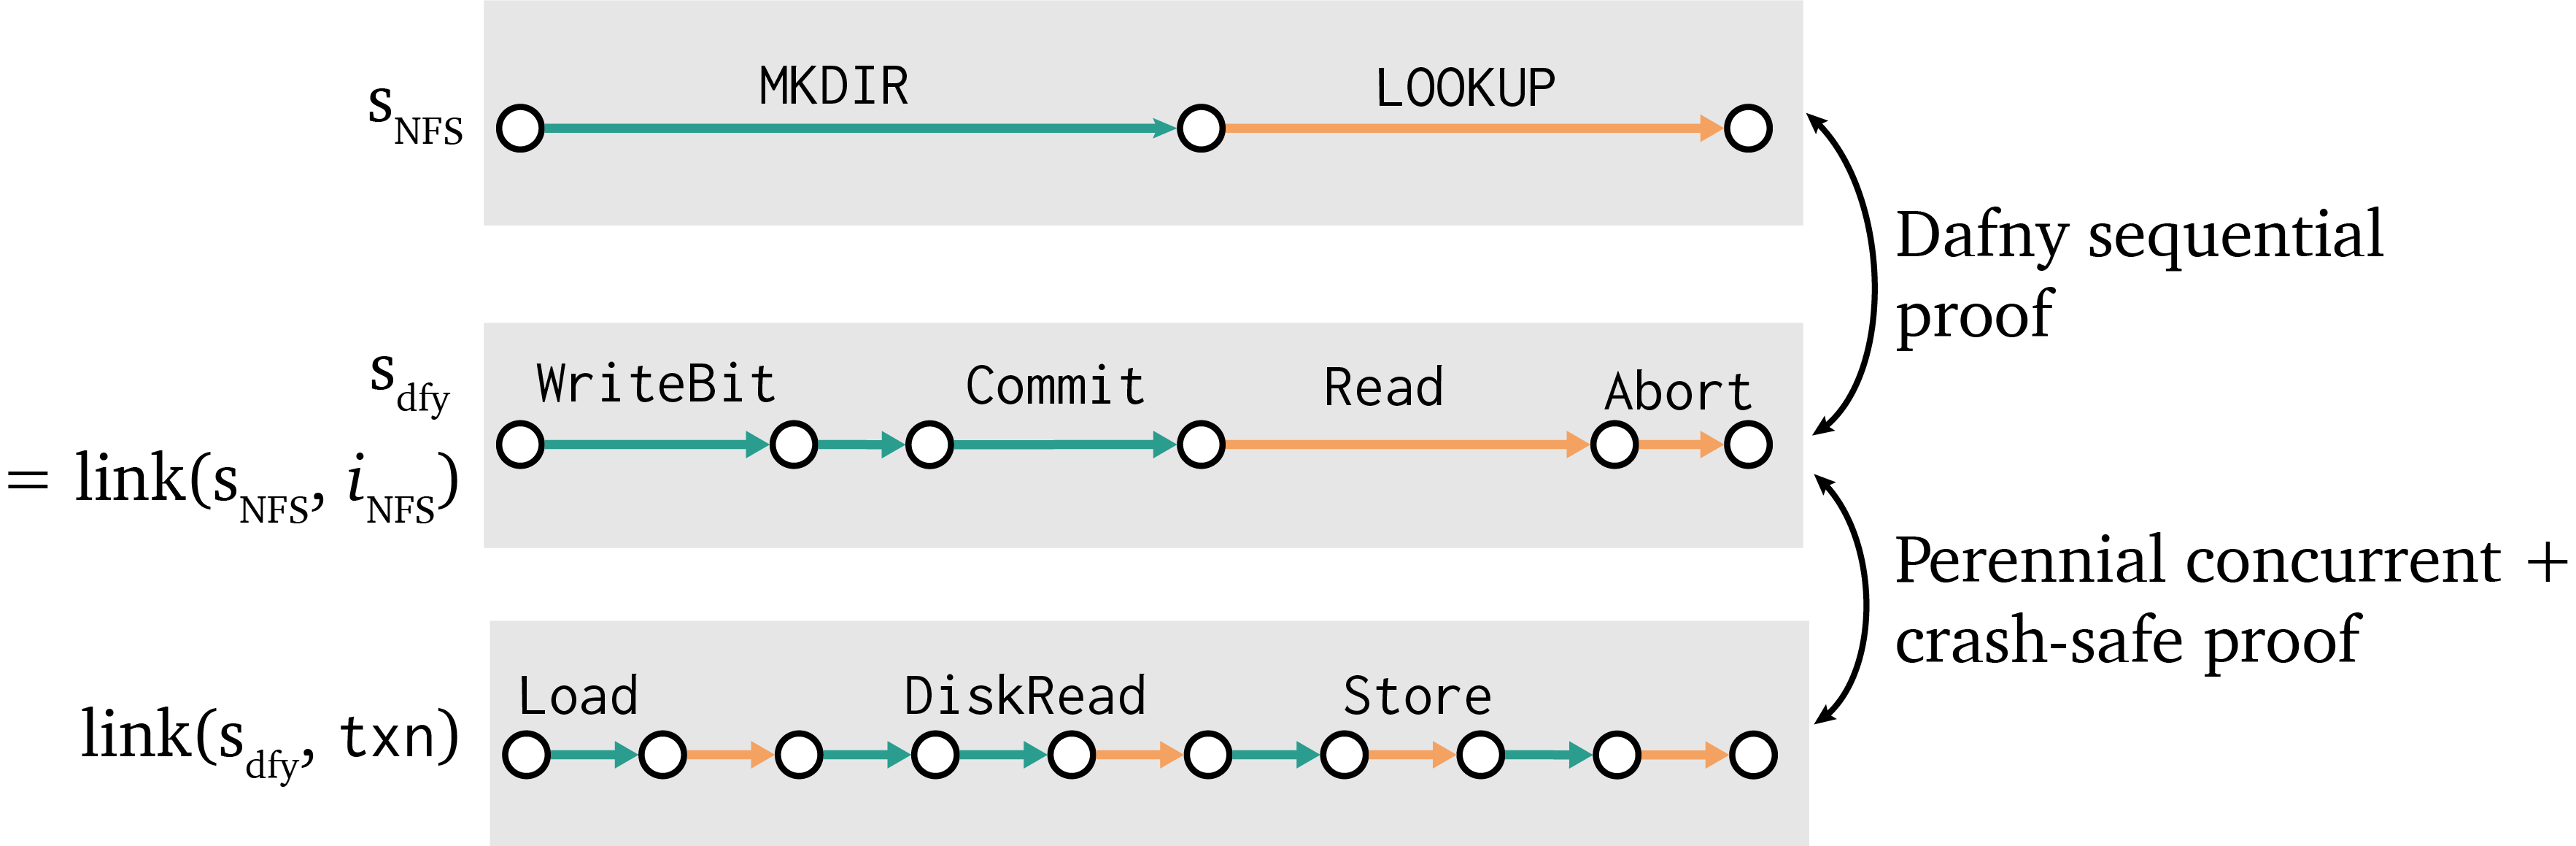
\includegraphics{fig/refinement-execs}
  \begin{center}
  \begin{tikzpicture}[scale=1, >=latex, every node/.append style={}]

  \tikzstyle{txnstate}=[circle,draw,minimum size=2mm,fill=blue!10]
  \tikzstyle{nfsstate}=[circle,draw,minimum size=2mm,fill=yellow!10]
  \tikzstyle{diskstate}=[circle,draw,minimum size=2mm,fill=green!10]
  \tikzstyle{switch}=[->, dashed, dash pattern=on 1.5pt off 2pt]
  \tikzstyle{stepr}=[thick,->]
  \tikzstyle{layer}=[font=\large]

  \setlength{\stepw}{1.25cm}
  \setlength{\dstepw}{\stepw*2}

  \newlength{\nfsbot}
  \newlength{\nfsmid}
  \setlength{\nfstop}{1.5cm}
  \setlength{\nfsbot}{.5cm}
  \setlength{\nfsmid}{(\nfstop+\nfsbot)/2}

  \newlength{\txntop}
  \newlength{\txnbot}
  \newlength{\txnmid}
  \setlength{\txntop}{-.5cm}
  \setlength{\txnbot}{-1.5cm}
  \setlength{\txnmid}{(\txntop+\txnbot)/2}

  \newlength{\disktop}
  \newlength{\diskbot}
  \newlength{\diskmid}
  \setlength{\disktop}{-2.5cm}
  \setlength{\diskbot}{-3.5cm}
  \setlength{\diskmid}{(\disktop+\diskbot)/2}

  \draw node (N0a) at (0,\nfstop) [nfsstate] {};
  \draw node (N1a) at (\dstepw,\nfstop) [nfsstate] {};
  \draw node (N1b) at (\dstepw,\nfsbot) [nfsstate] {};
  \draw node (N2b) at (\dstepw*2,\nfsbot) [nfsstate] {};

  \draw [stepr] (N0a.east) -- (N1a.west) node[midway,above=.2] {\code{LOOKUP}};
  \draw [stepr] (N1b.east) -- (N2b.west) node[midway,above=.2] {\code{CREATE}};
  \draw [switch] (N1a.south) -- (N1b.north);

  \draw node (T0a) at (0,\txntop) [txnstate] {};
  \draw node (T1a) at (\stepw,\txntop) [txnstate] {};
  \draw node (T2a) at (\stepw*2,\txntop) [txnstate] {};
  \draw node (T2b) at (\stepw*2,\txnbot) [txnstate] {};
  \draw node (T3b) at (\stepw*3,\txnbot) [txnstate] {};
  \draw node (T4b) at (\stepw*4,\txnbot) [txnstate] {};

  \draw [stepr] (T0a.east) -- (T1a.west) node[midway,above=.2] {};
  \draw [stepr] (T1a.east) -- (T2a.west) node[midway,above=.2] {\code{Commit}};
  \draw [switch] (T2a.south) -- (T2b.north);
  \draw [stepr] (T2b.east) -- (T3b.west) node[midway,above=.2] {};
  \draw [stepr] (T3b.east) -- (T4b.west) node[midway,above=.2] {\code{Abort}};

  \draw node (D0a) at (0,\disktop) [diskstate] {};
  \draw node (D1a) at (\stepw,\disktop) [diskstate] {};
  \draw node (D1b) at (\stepw,\diskbot) [diskstate] {};
  \draw node (D2b) at (\stepw*2,\diskbot) [diskstate] {};
  \draw node (D3b) at (\stepw*3,\diskbot) [diskstate] {};
  \draw node (D3a) at (\stepw*3,\disktop) [diskstate] {};
  \draw node (D4a) at (\stepw*4,\disktop) [diskstate] {};

  \draw [stepr] (D0a.east) -- (D1a.west) node[midway,above=.2] {\code{Read}};
  \draw [switch] (D1a.south) -- (D1b.north);
  \draw [stepr] (D1b.east) -- (D2b.west) node[midway,above=.2] {\code{Write}};
  \draw [stepr] (D2b.east) -- (D3b.west) node[midway,above=.2] {};
  \draw [switch] (D3b.north) -- (D3a.south);
  \draw [stepr] (D3a.east) -- (D4a.west) node[midway,above=.2] {};

  \draw [align=center] node (NFS) at (\stepw*5.5,\nfsmid) [layer] {$\snfs$ \\ \gooselayer{NFS}};
  \draw [align=center] node (Txn) at (\stepw*5.5,\txnmid) [layer] {$\sdfy$ \\ \gooselayer{Txn}};
  \draw [align=center] node (Disk) at (\stepw*5.5, \diskmid) [layer] {$\linkedcode$ \\ \gooselayer{Disk}};

\end{tikzpicture}

  \end{center}
  \caption[One execution of DaisyNFS at its three abstraction levels]{One possible execution of DaisyNFS, receiving parallel LOOKUP and
    CREATE operations, at its three abstraction levels.
    Within an execution each row is a thread, and dashed arrows indicate
    context switches.
    The proof shows the bottom execution is equivalent to an atomic execution of
    each thread at
    the Txn layer~(in \cref{thm:gotxn-transfer}),
    and sequential reasoning shows each atomic sequence behaves according to the NFS
    specification~(in \cref{thm:dafny}).}
  \label{fig:refinement-execs}
\end{figure}

There are two assumptions needed for the theorems to compose. First,
$\seqrefinement_{\mathrm{dfy}}(i_{NFS})$ should imply $\seqrefinement(i_{NFS})$,
to bridge the assumption and theorem being proven in Dafny. That is, the
encoding of the refinement conditions in Dafny must be correct, but also the
semantics of the transaction system operations modeled in Dafny must match the
Coq proof. Second, every Dafny transaction must be valid, meaning
$\mathrm{safe}(i_{NFS}(op))$. Safety has a static restriction that transactions
should not modify global state, which the Dafny code satisfies because the only
mutable state in the file-system Dafny class is the transaction system, so
file-system operations cannot make mutations other than through GoTxn. The
dynamic restrictions for safety are expressed with preconditions on the GoTxn
interface so that Dafny automatically enforces them.

\tej{subtlety about internal mutable state}

% We have some
% confidence this holds due to a simple check over the Dafny code: the only
% mutable state in the Dafny class that implements the file system is the ghost
% variables and the transaction system, so it cannot make mutations other than
% through GoTxn (ghost variables cannot influence execution due to the design of
% Dafny).

\section{Verifying the Dafny implementation}%
\label{sec:daisy:design}

\Cref{sec:daisy:proof-dafny}
explains how DaisyNFS connects sequential verification in Dafny to concurrency
and crash safety in GoTxn. This instead section focuses on the sequential
verification and file-system design themselves.

% The proof is given by annotating the code with proof steps, which include
% updates to ghost state, assertions to assist the automated verification, and
% calls to lemmas.

DaisyNFS is implemented and verified in several layers of abstraction, depicted
in \cref{fig:dafny-layers}. Each layer is implemented as a class that wraps the
lower layer as a field, until finally the transaction system is an assumed interface in Dafny.
The \cc{daisy-nfsd} binary implements the NFS wire protocol in
unverified Go code and calls the top-level Dafny class and its verified
methods to handle each operation.

\begin{figure}
\small \centering
\begin{tabular}{ll}
  \toprule
  \textbf{Layer} & \textbf{Functionality} \\
  \midrule
  daisy-nfsd & NFS wire protocol. \\
  dir & Directories and top-level NFS API. \\
  typed & Inode allocation. \\
  byte & Implement byte-level operations using blocks. \\
  block & Gather blocks for each file into a single sequence. \\
  indirect & Indirect blocks organized in a tree. \\
  inode & In-memory, high-level inodes; block allocation. \\
  txn & Assumed interface to external transaction system. \\
  \bottomrule
\end{tabular}
\caption{Layers in the Dafny implementation and proof of the file-system
operations.}
\label{fig:dafny-layers}
\end{figure}

The layers of the file system
can be organized into groups that implement three difficult pieces of
functionality: organizing data blocks into metadata and data (the
indirect and block layers), translating byte-level operations into
block operations (the byte and typed layers), and implementing
directories as special files that the file system itself reads and
writes (the dir layer). The modularity was essential to complete the proof in
manageable chunks (to avoid overwhelming the developer and prover), and it would
have been natural even without verification.

\subsection{Implementing the file system using transactions}

The design of DaisyNFS is broadly similar to the file system in xv6~\cite{xv6},
as well as Yggdrasil~\cite{sigurbjarnarson:yggdrasil}, a verified sequential
file system. We also adopt the recursive strategy for implementing and
verifying indirect blocks from DFSCQ~\cite{akonradi-meng}; recursion simplifies
the implementation of triply-indirect blocks, which are needed to reach a
reasonable maximum file size of 512GB.\@ Unlike most file systems, DaisyNFS is designed
to fit every operation into a transaction in order to support our goal of
sequential reasoning. This is a non-standard design and we encountered some
unique challenges in doing so. In this section we highlight difficulties in
fitting two features into transactions: rename and freeing space from deleted
files.

\subsubsection{Rename}
\label{sec:dafny:rename}

The NFS RENAME operation is similar to the \cc{rename} system call: it moves a
source file or directory to a destination location. What makes it tricky is that
it involves more than one inode and hence introduces the possibility for
deadlock.
% , which we would like to avoid even if the theorems do not forbid it.
We
use the standard strategy of enforcing a global ordering where inodes are always
locked in numerical order (smaller inode numbers first); this avoids a deadlock
where a cycle of threads is waiting on each other.

In a rename operation, the source and destination are each specified by a
combination of the parent directory inode and name within that directory. Rename
has an additional functionality of overwriting the destination if the source and
destination are files, or if both are directories and the destination is empty.
It is this latter check that makes deadlock avoidance difficult: it is necessary
to lock the source and destination directories first to lookup the source and
destination names, but those might be files that are earlier in the inode lock
order. We address this in the code by returning an error from the Dafny
transaction before the lock order would be violated. The error comes with the
set of inodes that should have been acquired.  The rename is then re-run with
this set of inodes as a lock hint which are all acquired in the correct
order at the beginning of the operation. The inodes to lock are only a hint and must be compared
against the current source and destination in case those inodes have changed in
the mean time. The rename operation runs in a loop until the lock hint succeeds;
the loop is potentially unbounded, but each iteration can only fail due to
concurrent renames that involve the same inodes.

At this point it is worth discussing the performance considerations that lead to
handling lock ordering in the file
system, rather than generically in GoTxn. The transaction system could
avoid deadlocks by either enforcing a global order over addresses or by
timing-out operations. Enforcing a global order is inefficient for the file
system; data blocks will never cause deadlock because the file system only
accesses a block after locking the (unique) inode that owns it. Timing-out
operations would lead to slow and spurious transaction failures that could more
rapidly be avoided in the higher-level code, hence we do not attempt to detect
deadlock dynamically.


\subsubsection{Freeing space}
\label{sec:dafny:freeing}

Freeing space becomes surprisingly tricky with large files. The problem is that
a large-enough file may reference too many blocks to be
freed in a single transaction. Transactions are bounded by the size of the
on-disk log (which can hold 511 blocks), whereas freeing a file requires
writing 0s to the block allocator for all of its formerly used blocks to mark them as free.
DaisyNFS handles this issue by splitting file removal and space reclamation
into separate transactions. The latter is implemented with an operation
\cc{ZeroFreeSpace(ino)} which frees and zeros the unused space in an inode that
we prove has no effect on the logical file-system state. Because this operation is a
logical no-op, it is safe to call it at any time.

The implementation is careful to call \cc{ZeroFreeSpace} after any operation
that leaves unused blocks, in particular \cc{REMOVE}, which deletes a file, and
\cc{SETATTR}, which can shrink a file by reducing its size. Since
\cc{ZeroFreeSpace} doesn't affect the user-visible data, it can return early to
avoid overflowing a transaction. The unverified code that manages freeing space
runs the operation in a loop until it covers all of the unused space in an
inode.

There is one case where freeing blocks is important for correctness and not just
to reclaim space. Growing a file is supposed to logically fill the new space
with zeros. If the file had old data in that space, it might not be zero but
instead contain previously written and deleted data, which both violates the specification and
is a potential security risk. The way we handle this with background freeing is
with validation: when the \cc{SETATTR} operation grows a file, it checks if the
free space is already zero first, and if not fails with a special error code. The
unverified code uses this error as a signal to immediately call
\cc{ZeroFreeSpace} and try the operation again. The same support also handles
holes created by writing past the end of a file, which are similarly supposed to
be zero.

The freeing implementation is an interesting example of using validation in
verification. The specification for much of the freeing code is loose, allowing
any data to be written to the free space. Only the code that checks if the
zeroing is done needs to be verified against a strong specification. The rest of
the code does still needs to be correct for this check to succeed, but we
aren't required to prove it.

\subsection{Verifying the indirect block implementation}%
\label{sec:dafny:indirect}

DaisyNFS supports large files using indirect blocks. A file's inode has a fixed
number of addresses for block addresses, some of which are used as indirect
blocks that hold another layer of addresses rather than direct blocks that have
file data. A single level of indirection is insufficient for a practical file
system, so DaisyNFS implements support for arbitrarily indirect blocks, and in
practice the file system uses up to triply-indirect blocks to support files up
to 512GB.\@

The indirect and block layers together implement an abstraction of a file as a
sequence of blocks, hiding the fact that some of the blocks are used as
metadata. These sequences are always of the maximum size, and only the next
layer reasons about file sizes. To efficiently represent files of the maximum
size, the code uses a convention that a zero block address is treated implicitly
as encoding a zero block, including for indirect blocks, an idea borrowed from
DFSCQ~\cite{akonradi-meng}. Indirect blocks are implemented recursively, where a
$k$-indirect block is always treated as containing 512 pointers to
$(k-1)$-indirect blocks, and a 0-indirect block contains file data. Zeros are
also treated recursively so that a single zero in an inode for the root of a
triply-indirect block efficiently stores a whole tree corresponding to many
gigabytes of zeros.

An inode has space for twelve 64-bit block addresses, after accounting for space
used by its attributes and type information. In principle all of these addresses
could be uniformly used as triply-indirect blocks. However, this would create a
lot of indirection for small files and lower performance for the common case.
Thus instead of organizing them in this way, the code uses a whole range, with
mostly direct blocks and a handful of indirect blocks. To keep the code general,
the indirection level of each of the twelve blocks is given in a global
indirect-block configuration, and most of the code is generic over the configuration. We currently
configure DaisyNFS with 8 direct blocks, two 1-indirect blocks, a 2-indirect
block, and a 3-indirect block. Just the direct and indirect blocks can address 4
MB fairly efficiently, but the triply-indirect block allows files to be large.

Indirect blocks pose a challenge for verification due to the classic problem of
\emph{aliasing}. The proof must show that modifying a data block or indirect
block has no effect on other files. In the DFSCQ proof, the invariant
captures the non-aliasing between files using separation logic, which makes
disjointness easy to express. In Dafny we have no such logical
technique, so we instead use a standard SMT-friendly trick for the invariant: in
addition to the physical mapping that tracks how to dereference a block address,
the indirect layer proof tracks a ghost \emph{reverse} mapping that tracks where
each in-use block number is stored. The invariant states that the forward and reverse
mappings are inverses of each other, which implies that modifying an address
only affects its owner and nothing else.

To encode the reverse mapping, the code uses a ``position'' datatype \cc{Pos} to
represent the location of a block within an inode. With indirect blocks, the
metadata blocks themselves also need to be considered locations, since the
invariant must also rule out metadata aliasing with data or other metadata. A
\cc{Pos} encodes an inode, an indirection level, and an offset for the blocks at
that indirection level to uniquely identify where a block is used. If we imagine
that an inode's block pointers are organized in a tree, the roots are stored
directly in the inode while the leaves are direct blocks. An indirection level
which is higher than the leaf level describes a metadata block.

The indirect block proof is split into the indirect and blocks layers. In the
indirect layer, the abstract state maps a \cc{Pos} to a block, and separately
tracks the size and attributes of each inode. The invariant also expresses that
the block allocator's used blocks have an associated \cc{Pos} and that the free
ones do not. The interface for the indirect layer exposes reads and writes for
positions, regardless of whether they are metadata or data blocks. The block
layer above instead exposes a map from inode number to a flat sequence of blocks by
mapping each leaf position to its linear index within the inode. Separating
these two made it easier to work on the indirect layer while exposing a much
more natural abstraction of a file as a sequence of blocks for the rest of the
file-system implementation.


% \subsection{Random notes on development process}
%
% \begin{itemize}
%   \item Used inefficient functional Dafny code at first, then slowly migrated to
%         in-memory data structures and improved performance.
%   \item Hard to debug and fix timeouts. Profiling verification performance is
%         hard.
%   \item Profiling Go code is great as usual. The generated code looks strange,
%         but I think after code generation it's pretty ordinary (the weird things
%         are mostly bad variable names, lot of unused assignments, and anonymous
%         functions that are immediately called).
%   \item Used some unit tests, but very few and only at the top level. Mainly
%         debugged Go compilation issues and cases where errors were
%         unintentionally being returned.
%   \item Trusted code isn't easy, had bugs in it before testing it thoroughly.
%         Also violated preconditions in top-level specs, triggering memory-safety
%         bugs.
% \end{itemize}

% \section{Proof of refinement for \sys}
\label{appendix:proof}

% make theorem re-statements get the same numbers
\setcounter{theorem}{0}

Previously in \autoref{sec:proof} we gave an informal overview of \sys's
correctness proof. This section develops the proof in more detail. There are two
gaps we will fill in compared to the proof above: first, we will be more precise
about what the requirements of the transaction system proof are and why DaisyNFS
satisfies them, and second, we will specify what the theorem says about recovery.

To make this section self-contained, we will re-state theorems 1--3 (with slight
tweaks to describe initialization better). First, we re-state program refinement
for the transaction system:

\begin{theorem}
  The transaction system's implementation $\txncode$ is a program refinement,
  meaning for all $p : \gooselayer{Txn}$, if $\mathrm{safe}(p)$, then
  $\mathrm{link}(p, \txncode) \refines p$. Initialization relates an all-zero
  disk to an all-zero transactional disk.
  \label{thm:txn-appendix}
\end{theorem}

So far, we have been vague about what exactly $p : \gooselayer{L}$ means. In
Coq, $\gooselayer{L}$ is a datatype in a language we called GooseLang, which is
intended to represent a Go program with access to operations from layer $L$. Any
GooseLang program has access to standard Go constructs like heap allocation,
concurrency, and operations on basic types like integers and booleans. All of
the concrete GooseLang code we reason about for the transaction system is in
$\gooselayer{Disk}$. $\gooselayer{Txn}$ is used to give a specification for code
using the transaction system, while $\gooselayer{NFS}$ is only used to model the
NFS server in the top-level specification.

The overall correctness statement for DaisyNFS refers to
$\stxn : \gooselayer{Txn}$, which models the Dafny implementation at the level
of transactions. We express the result from Dafny as the following refinement
theorem:

\begin{theorem}
  $\sdfy \refines \snfs$. Initialization requires an invariant stated in Dafny,
  which is established by running a separate \cc{Init} procedure verified in
  Dafny starting from an all-zero transactional disk.
  \label{thm:dafny}
\end{theorem}

The overall correctness theorem says
$\linkedcode \refines \snfs$ (ignoring initialization). Both the code and spec
are expressed as a single program, a top-level loop whose
observable behavior is to receive some input from the outside world, which is an
NFS operation and its arguments, then to dispatch a handler thread to process
the request and respond over the network with the handler's result. The
difference between the two is that the specification $\snfs$ processes requests
atomically and according to a high-level NFS transition system, whereas in the
code $\linkedcode$ handlers represent the executable code running on top of a
disk, derived by compiled from Dafny and linking with the transaction-system
implementation.

Notice that even the code dispatch loop in this specification abstracts over the
details of interacting with the outside world; in reality, the executable binary connects
to clients over TCP and parses a stream of bytes to produce NFS operations. The
NFS wire protocol is outside the scope of our verification. We want to
interpret the specification as saying something about the binary that we run at
the end of the day; in doing so, we assume that the code correctly implements
the protocol, translating the byte stream into the right method calls for each
handler, and then translating the responses back.

Combining the above results, the top-level specification is:

\begin{theorem}
  $\linkedcode \refines \snfs$. Initialization requires
  starting from an empty disk, then running the initialization implemented in
  Dafny. After that, the system boots by first recovering the transaction
  system's state, then running file-system recovery.
  \label{thm:correctness}
\end{theorem}

Recovery is part of this specification because the semantics of running any
program includes the possibility to crash and restart, with a crash considered
visible behavior. With crashing as just another possible behavior, the normal
definition of refinement enforces that $\linkedcode$ has crash atomicity, since
its crash and restart behaviors must correspond to one from $\snfs$ which does
not allow crashes during a transaction.

The overall strategy to prove this theorem is
$\linkedcode \refines \sdfy \refines \snfs$; refinement is clearly transitive
because it is a subset relation on program behaviors. This argument
centers on $\sdfy : \gooselayer{Txn}$. Note that we are assuming that
such a program actually exists, one that models the Dafny code using GooseLang
--- it isn't something we'll actually construct because we don't translate Dafny
to GooseLang. We believe this assumption is reasonable because GooseLang is
fairly complete and we use only basic features of Go to implement the file
system. At this level of abstraction, transactions are not represented with the
usual \cc{Begin}, \cc{Commit}, and \cc{Abort} calls but with a
specification-only Atomically operation.

In the following two sections we expand on how to apply \autoref{thm:txn} to
$\sdfy$ and how the initialization and recovery code is incorporated to prove
\autoref{thm:correctness}.

\subsection{Safety}

The formal definition of safety in Coq is split into two properties. The first
is a static restriction that describes the
relationship between the specification's $\mathrm{Atomically}(f)$ construct and
the code that implements a transaction. Static restrictions rule out constructs
that would break atomicity, notably use of the heap could produce effects
outside the transaction system. They also enforce a correct discipline over
transaction objects; for example, a single transaction should use only one
\cc{tx} object and when finished should call one of \cc{Commit} or \cc{Abort}
and then dispose of \cc{tx}. The translation of a transaction body is
non-trivial because the specification has operations that implicitly refer to
the ``current'' transaction, while the code must manipulate a transaction object
\cc{tx}. The Coq implementation enforces the static restrictions using a type
system, which allows us to prove program refinement
using a standard proof technique called \emph{logical relations}.

The model of the Dafny code $\sdfy$ uses Atomically blocks, but its
implementation uses the usual transaction-system API\@. We can be fairly confident
that the real Dafny code after linking with Go is equivalent to $\linkedcode$.
The main requirement is that the Dafny code manage transaction objects the same
way as the type system does. Each handler is written as a method that takes a
transaction object (and it never starts another transaction) and returns a
result or signals an error. Then a common utility function \cc{runTxn(f)} takes
care of beginning a transaction, passing it to \cc{f}, and determining whether
to commit or abort based on the return value. This utility function captures
exactly the translation of an Atomically block in the transaction system specification.

The more serious restriction is that transactions cannot access the heap at all.
The Dafny code does use the heap, but only ever in a local way to access objects
allocated earlier in the transaction. We can justify this in the proof by
distinguishing $\sdfy$, which is as faithful to the syntactic Dafny code as
possible, from a program $\sdfyAlt$ that is equivalent to $\sdfy$ but where the
use of the heap has been eliminated. $\sdfyAlt$ can be constructed from $\sdfy$
by using a state monad to turn every heap access into purely functional code.
We expect such a construction to succeed because
a simple audit shows that the Dafny code is in a class that has no mutable
variables other than the transaction system and ghost variables,
so it is impossible for a transaction to have a non-local effect.

Applying \autoref{thm:txn} to this revised Dafny program, we obtain that
$\linked{\sdfyAlt} \refines \sdfyAlt$. Given that $\sdfyAlt \progeq \sdfy$, it is
reasonable that the linked versions are also equivalent, completing the first
part of the refinement proof:
\[
  \linked{\sdfy} \progeq \linked{\sdfyAlt} \refines \sdfyAlt \progeq \sdfy
\]

The other side of the refinement comes from reasoning about $\sdfy$ in Dafny.
The theorems proven in Dafny imply that $\sdfy \refines \snfs$. Reasoning about
refinement between these two programs is simple because the granularity of their
concurrency is the same: both have the same structure, but $\sdfy$ executes a
whole implementation for each transaction while $\snfs$ has only one transition.
The Dafny proofs show that $\sdfy$ maintains ghost state corresponding to the
NFS transition system and an invariant that is strong enough to conclude all the
handlers simulate the NFS specification.

There is one subtlety in connecting this proof to the transaction system proof,
even though it appears to be simple transitivity to connect them and show
$\linkedcode \refines \snfs$. The subtlety is that the Dafny proof is about a
model of the transaction system expressed in Dafny, whereas the transaction
system's program refinement proof uses a specification written in Coq. It is
important that the specifications line up, or at least that the behaviors in Coq
are a subset of those in Dafny. These being different formal systems we cannot
directly compare them, but we aimed to formalize the two as closely as possible.
The interfaces are also sufficiently narrow that we can inspect and compare both
by hand.

We have discussed the static restrictions for a safe Txn program, but there are
also dynamic restrictions, namely that the caller should not trigger undefined
behavior in the transaction system. We handle this systematically by enforcing
all of the required preconditions in the Dafny interface to the transaction
system, and these preconditions are respected by virtue of the Dafny proof
succeeding. Similar to trusting that the semantics of the transaction system are
the same, we also trust that Dafny enforces the preconditions correctly.

\subsection{Initialization and recovery}

So far, when we write a refinement of the form $\sdfy \refines \snfs$, we have
been vague about how initialization and recovery factor in. Now we'll
be more precise about how these are handled, first in the program refinement
definition for the transaction system and then for the overall DaisyNFS
correctness theorem.

The transaction system does not require any initialization code, as long as the
disk is initially all-zero. The theorem relates an all-zero disk to a
transaction-system state full of zero objects. Our proof requires the caller to
use each disk block with a consistent object size (since changes in object size
are difficult to coordinate between threads). We call a mapping of block numbers
to object sizes a \emph{schema}, and enforce that the schema picked during
initialization is static for the rest of the execution. The Dafny interface also
uses a constant schema, which DaisyNFS sets to include a super block, some
number of inode blocks, then some allocator blocks, and finally data blocks
for the remainder of the disk.

Unlike the transaction system, the file system does require initialization code
separate from recovery, because an all-zero set of objects is not a valid
file-system state (at minimum, the root inode should be an allocated directory).
More precisely then, DaisyNFS's specification as stated above requires that the
caller first run \cc{Init} on an all-zero disk, initially establishing the
file-system invariant. After that, the system should run the recovery method on
each reboot to behave like $\sdfy$ according to \autoref{thm:txn}.

While we can use \autoref{thm:txn} to show the code behaves like $\sdfy$, why
does $\sdfy$ behave like $\snfs$ across a crash? The specification we prove in
Dafny about recovery is this:

\begin{verbatim}
constructor Recover(txs: TxnSystem,
    ghost fs: Filesys)
  requires fs.Valid()
  requires same_txn_disk(txs, fs.txs)
  ensures this.data == fs.data
  ensures Valid()
\end{verbatim}

The key to this proof is the argument \texttt{fs: Filesys}, which encodes the
assumptions about the file system just before the crash. Because this file
system is now lost, it is a \emph{ghost} argument; we cannot implement recovery
using the
old in-memory state, but do get to assume that the transaction system \cc{txs}
is the same as before the crash. Each operation is handled
atomically, so recovery also assumes that the file system satisfies its
\cc{fs.Valid()} invariant. What we prove in this specification Dafny
is that \cc{Recover()} produces a new, valid \cc{Filesys} in memory with the
same abstract state as the old one. With the file-system invariant restored, we
can say that operations after a crash and recovery continue to follow the NFS
state machine.

\subsection{A hypothetical mechanized proof}

One question one might have is why this proof needs to happen on paper. The
agenda for mechanizing it would look something like this: compile the Dafny code
to Go, then abstract away the details of the network interaction to produce
$\server_{\mathrm{code}}$. The same compiled code also gives an explicit
definition of $\sdfy$ where we use Atomically to wrap each transaction. Then, we
might give explicit definitions for each intermediate step, in particular
$\sdfyAlt$ and its compiled version $\linkedcode$. We would prove that
$\sdfyAlt$ is safe; perhaps we could assume dynamic safety of $\sdfy$, trusting
that part to the Dafny proof. We could then show in Coq that
$\server_{\mathrm{code}} \approx \linkedcode \refines \sdfyAlt \equiv \sdfy$,
applying Theorem 1 for the middle step.

There are many barriers to this process. The first is that Goose cannot
translate all of the patterns produced by the Dafny compiler in order to
initially import the Dafny code into Coq. The second is that $\sdfyAlt$ is a
non-trivial transformation of $\sdfy$ to really carry out. Finally, even after
constructing the intermediate programs we would need infrastructure for
reasoning about program equivalences in GooseLang. All of these are surmountable
problems, but it is unlikely that they increase confidence in the proof beyond
careful manual inspection.

